\documentclass{article}

\usepackage{tikz}
\usepackage{commath}

\begin{document}
	\begin{center}
		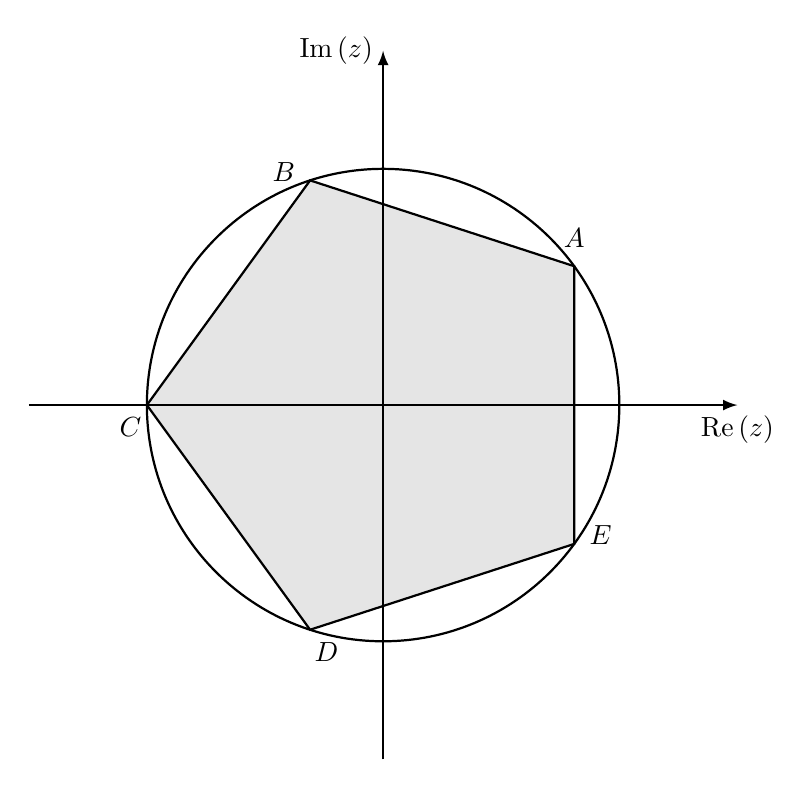
\begin{tikzpicture}[scale=3]			
			\draw[thick, fill=gray!20] (180:1) 
				\foreach \i/\l in {1/D, 2/E, 3/A, 4/B, 5/C } {
					 -- (180 + \i*360/5:1) node[pos=1.1]{\(\l\)}
				};
			\draw[thick] (0,0) circle (1cm);
			
			\draw[thick, ->, >=latex] (-1.5,0) -- (1.5,0) 
				node[below]{\(\operatorname{Re} \left(z\right)\)};
			\draw[thick, ->, >=latex] (0,-1.5) -- (0,1.5) 
				node[left]{\(\operatorname{Im} \left(z\right)\)};
		\end{tikzpicture}
	\end{center}
\end{document}